Ein LC-Schwingkreis besteht aus einer Spule mit der Induktivität $L$ und einem Kondensator mit der Kapazität $C$. Die Spule speichert ein magnetisches Feld 
\todo[]{Ich finde speichern ist hier für das magnetische Feld nicht ganz das richtige Wort}
und der Kondensator ein elektrisches. In dem Schwingkreis wechseln sich beide Felder periodisch ab mit der Folge, dass sich der Stromfluss  mit gleicher Periode umkehrt. Zwei LC-Schwingkreise können durch einen weiteren Kondensator $C_\text{K}$ gekoppelt werden (siehe Abbildung \ref{fig:Abb2}).
\begin{figure}[h!]
	\centering
	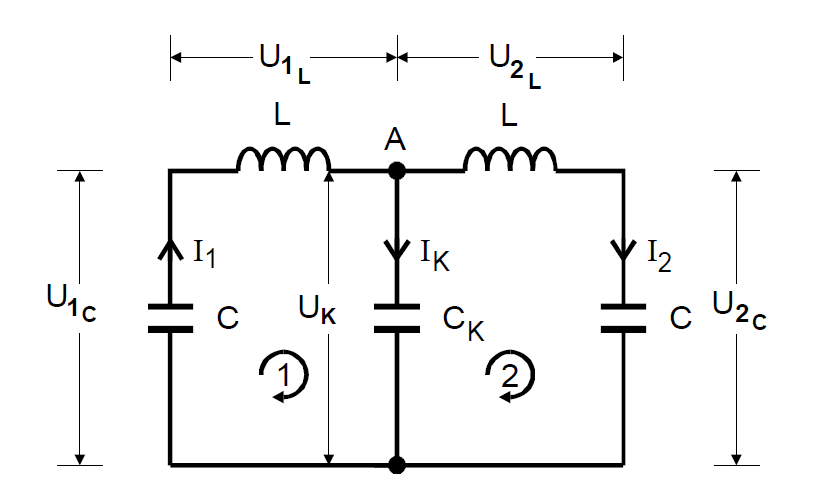
\includegraphics[width=0.7\textwidth]{Abb2.png}
	\caption{Gekoppelter LC-Schwingkreis}
	\label{fig:Abb2}
\end{figure} \\
Der Stromfluss in den einzelnen Kreisen wird durch die Kirchhoffschen Regeln bestimmt.
\begin{align}
I_\text{K} = I_\text{1}-I_\text{2} \\
U_\text{1C} + U_\text{1L} + U_\text{K} = 0 \\
U_\text{2C} + U_\text{2L} + U_\text{K} = 0
\end{align}
Die gekoppelten Differentialgleichungen für beide Schwingkreise folgen mit
\begin{align}
U_\text{C} = \frac{1}{C} \int I \dd t \quad \text{und} \quad U_\text{L} = L \dv{I}{x} \quad :  \\
\text{1. DGL:} \quad L \dv[2]{I_1}{x} + \frac{1}{C} I_1 + \frac{1}{C_\text{K}}(I_1 + I_2) = 0 \\
\text{2. DGL:} \quad L \dv[2]{I_2}{x} + \frac{1}{C} I_2 - \frac{1}{C_\text{K}} (I_1 + I_2) = 0
\end{align}
Durch entkoppeln der Differentialgleichungen folgen Lösungen für die einzelnen Ströme $I_1$ und $I_2$ mit den Frequenzen $\nu^+$ und $\nu^-$. Die Lösungen sind zudem abhängig von den Anfangsamplituden $I_{10}$ des erstem Schwingkreises und $I_{20}$ des zweiten Schwingkreises.
\begin{align}
I_1(t) = \frac{1}{2}(I_{10} + I_{20}) \cos(2 \pi \nu^+ t) + \frac{1}{2}(I_{10} - I_{20}) \cos(2 \pi \nu^- t) \\
I_2(t) = \frac{1}{2}(I_{10} + I_{20}) \cos(2 \pi \nu^+ t) - \frac{1}{2}(I_{10} - I_{20}) \cos(2 \pi \nu^- t)
\end{align}
Die Frequenzen sind dabei
\begin{align}
\nu^+ = \frac{1}{2 \pi \sqrt{L C}} \quad \text{und} \label{Frequenz_p} \\
\nu^- = \frac{1}{2 \pi \sqrt{L\left(\frac{1}{C} + \frac{2}{C_\text{K}}\right)^{-1}}} \quad . \label{Frequenz_m}
\end{align}
Nun werden wichtige Spezialfälle dieses komplexen Verhaltens beschrieben. Die zwei \textbf{Fundamentalschwingungen} zeichnen sich dadurch aus, dass die Anfangsamplituden $I_{10}$ und $I_{20}$ gleich groß sind ($\abs{I_{10}} = \abs{I_{20}}$). Sind beide Schwingkreis in Phase ($I_{10}=I_{20}$) schwingen sie mit der Frequenz $\nu^+$. Der Koppelkondensator hat hier keine Funktion. Er ist zu keinem Zeitpunkt geladen. Der Schwingkreis verhält sich wie ein einfacher LC-Kreis. Sind die Schwingkreise um eine halbe Periode phasenverschoben ($I_{10} = - I_{20}$) schwingen sie mit der etwas höheren Frequenz $\nu^-$. Die höhere Frequenz entsteht dadurch, dass der Koppelkondensator einem periodisch wechselnden Stromfluss ausgesetzt ist und die anderen beiden Kondensatoren unterstützt. \\
Das Phänomen der \textbf{Schwebung} tritt auf, wenn einer der Kreise stimuliert wird bzw. eine Anfangsamplitude hat und der andere Kreis keine Anfangsamplitude aufweist.
\todo[color=green]{Perfekt. Mir ist nur gerade aufgefallen, dass man das hier gar nicht verwendet. Man setzt einfach $I_{20}=0$ und benutzt dann ein Additionstheorem. Die Frequenzen spielen da gar keine Rolle.}
\todo{Stimmt!}
\begin{align}\label{Schwebung}
	I_1(t) = I_{10}  \cos \left( \pi (\nu^+ + \nu^-) t \right) \cdot  \cos \left( \pi (\nu^+ - \nu^-) t \right) \\
	I_2 (t) = I_{10}  \sin \left( \pi (\nu^+ + \nu^-) t \right) \cdot  \sin \left( \pi (\nu^+ - \nu^-) t \right) 
\end{align}
Es entsteht eine Schwingung (siehe Abbildung \ref{fig:Abb3})  mit den Frequenzen der einzelnen Schwingkreise
\begin{equation}
	\nu = \frac{1}{2} (\nu^+ + \nu^-)
\end{equation}
und einer Schwebungsfrequenz von 
\todo[color=red, inline]{Der hintere Cosinus/ Sinus ist doch jeweils für die große Schwingung, also die, die die Schwebungsbäuche beschreibt, verantwortlich. Die Kreisfrequenz ist da $\omega = \pi(\nu^+-\nu^-)$. Für die richtige Frequenz $f$ gilt doch aber $f=\frac{\omega}{2\pi}=\frac{(\nu^+-\nu^-)}{2}$?}
\todo[color=green, inline]{Das mit der Frequenz ist ein wichtiger Punkt. ich habe es bei beiden Gleichungen geändert - dann ist es auch so wie in der Anleitung. Die Freqenz der Schebung ist allerdings wirklich so, da die Frequenz von $\abs{\sin\frac{(\nu^+-\nu^-)}{2}}$ doppelt so groß ist wie die von $\sin\frac{(\nu^+-\nu^-)}{2}$. In Abbildung zwei sieht man das ganz schön.}
\begin{equation}
	f =  (\nu^+ - \nu^-) \quad .
\end{equation}
Es handelt sich um einen periodischen Energieaustausch zwischen den beiden Schwingkreisen mit der Schwebungsfrequenz.
 \begin{figure}[h!]
 	\centering
 	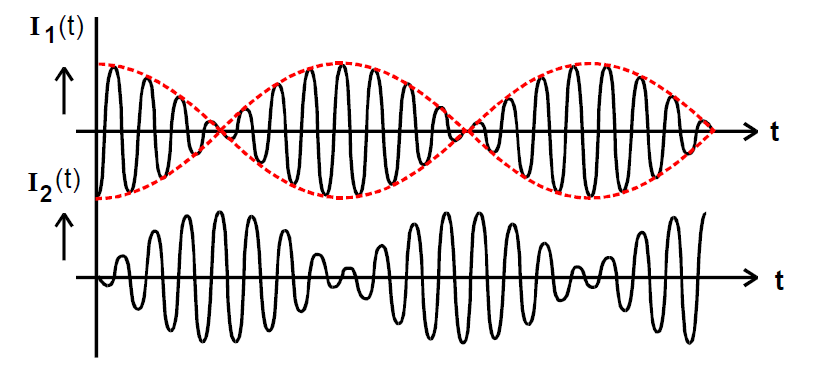
\includegraphics[width=0.7\textwidth]{Abb3.png}
 	\caption{Stromveräufe beider Schwingkreise im Fall der Schwebung}
 	\label{fig:Abb3}
 \end{figure}